
%% bare_jrnl_compsoc.tex
%% V1.4a
%% 2014/09/17
%% by Michael Shell
%% See:
%% http://www.michaelshell.org/
%% for current contact information.
%%
%% This is a skeleton file demonstrating the use of IEEEtran.cls
%% (requires IEEEtran.cls version 1.8a or later) with an IEEE
%% Computer Society journal paper.
%%
%% Support sites:
%% http://www.michaelshell.org/tex/ieeetran/
%% http://www.ctan.org/tex-archive/macros/latex/contrib/IEEEtran/
%% and
%% http://www.ieee.org/

%%*************************************************************************
%% Legal Notice:
%% This code is offered as-is without any warranty either expressed or
%% implied; without even the implied warranty of MERCHANTABILITY or
%% FITNESS FOR A PARTICULAR PURPOSE!
%% User assumes all risk.
%% In no event shall IEEE or any contributor to this code be liable for
%% any damages or losses, including, but not limited to, incidental,
%% consequential, or any other damages, resulting from the use or misuse
%% of any information contained here.
%%
%% All comments are the opinions of their respective authors and are not
%% necessarily endorsed by the IEEE.
%%
%% This work is distributed under the LaTeX Project Public License (LPPL)
%% ( http://www.latex-project.org/ ) version 1.3, and may be freely used,
%% distributed and modified. A copy of the LPPL, version 1.3, is included
%% in the base LaTeX documentation of all distributions of LaTeX released
%% 2003/12/01 or later.
%% Retain all contribution notices and credits.
%% ** Modified files should be clearly indicated as such, including  **
%% ** renaming them and changing author support contact information. **
%%
%% File list of work: IEEEtran.cls, IEEEtran_HOWTO.pdf, bare_adv.tex,
%%                    bare_conf.tex, bare_jrnl.tex, bare_conf_compsoc.tex,
%%                    bare_jrnl_compsoc.tex, bare_jrnl_transmag.tex
%%*************************************************************************


% *** Authors should verify (and, if needed, correct) their LaTeX system  ***
% *** with the testflow diagnostic prior to trusting their LaTeX platform ***
% *** with production work. IEEE's font choices and paper sizes can       ***
% *** trigger bugs that do not appear when using other class files.       ***                          ***
% The testflow support page is at:
% http://www.michaelshell.org/tex/testflow/


\documentclass[10pt,journal,compsoc]{IEEEtran}
%
% If IEEEtran.cls has not been installed into the LaTeX system files,
% manually specify the path to it like:
% \documentclass[10pt,journal,compsoc]{../sty/IEEEtran}
\usepackage{graphicx}
\usepackage[linesnumbered,ruled]{algorithm2e}
\usepackage{url}
\usepackage{epstopdf}
\usepackage{indentfirst}
\usepackage[tight,footnotesize]{subfigure}
\usepackage{amsmath}
\usepackage{amssymb}
\usepackage{multirow}
\usepackage{color}
\usepackage{CJK}

\newtheorem{Lemma}{Lemma}




% Some very useful LaTeX packages include:
% (uncomment the ones you want to load)


% *** MISC UTILITY PACKAGES ***
%
%\usepackage{ifpdf}
% Heiko Oberdiek's ifpdf.sty is very useful if you need conditional
% compilation based on whether the output is pdf or dvi.
% usage:
% \ifpdf
%   % pdf code
% \else
%   % dvi code
% \fi
% The latest version of ifpdf.sty can be obtained from:
% http://www.ctan.org/tex-archive/macros/latex/contrib/oberdiek/
% Also, note that IEEEtran.cls V1.7 and later provides a builtin
% \ifCLASSINFOpdf conditional that works the same way.
% When switching from latex to pdflatex and vice-versa, the compiler may
% have to be run twice to clear warning/error messages.






% *** CITATION PACKAGES ***
%
\ifCLASSOPTIONcompsoc
  % IEEE Computer Society needs nocompress option
  % requires cite.sty v4.0 or later (November 2003)
  \usepackage[nocompress]{cite}
\else
  % normal IEEE
  \usepackage{cite}
\fi
% cite.sty was written by Donald Arseneau
% V1.6 and later of IEEEtran pre-defines the format of the cite.sty package
% \cite{} output to follow that of IEEE. Loading the cite package will
% result in citation numbers being automatically sorted and properly
% "compressed/ranged". e.g., [1], [9], [2], [7], [5], [6] without using
% cite.sty will become [1], [2], [5]--[7], [9] using cite.sty. cite.sty's
% \cite will automatically add leading space, if needed. Use cite.sty's
% noadjust option (cite.sty V3.8 and later) if you want to turn this off
% such as if a citation ever needs to be enclosed in parenthesis.
% cite.sty is already installed on most LaTeX systems. Be sure and use
% version 5.0 (2009-03-20) and later if using hyperref.sty.
% The latest version can be obtained at:
% http://www.ctan.org/tex-archive/macros/latex/contrib/cite/
% The documentation is contained in the cite.sty file itself.
%
% Note that some packages require special options to format as the Computer
% Society requires. In particular, Computer Society  papers do not use
% compressed citation ranges as is done in typical IEEE papers
% (e.g., [1]-[4]). Instead, they list every citation separately in order
% (e.g., [1], [2], [3], [4]). To get the latter we need to load the cite
% package with the nocompress option which is supported by cite.sty v4.0
% and later. Note also the use of a CLASSOPTION conditional provided by
% IEEEtran.cls V1.7 and later.





% *** GRAPHICS RELATED PACKAGES ***
%
\ifCLASSINFOpdf
  % \usepackage[pdftex]{graphicx}
  % declare the path(s) where your graphic files are
  % \graphicspath{{../pdf/}{../jpeg/}}
  % and their extensions so you won't have to specify these with
  % every instance of \includegraphics
  % \DeclareGraphicsExtensions{.pdf,.jpeg,.png}
\else
  % or other class option (dvipsone, dvipdf, if not using dvips). graphicx
  % will default to the driver specified in the system graphics.cfg if no
  % driver is specified.
  % \usepackage[dvips]{graphicx}
  % declare the path(s) where your graphic files are
  % \graphicspath{{../eps/}}
  % and their extensions so you won't have to specify these with
  % every instance of \includegraphics
  % \DeclareGraphicsExtensions{.eps}
\fi
% graphicx was written by David Carlisle and Sebastian Rahtz. It is
% required if you want graphics, photos, etc. graphicx.sty is already
% installed on most LaTeX systems. The latest version and documentation
% can be obtained at:
% http://www.ctan.org/tex-archive/macros/latex/required/graphics/
% Another good source of documentation is "Using Imported Graphics in
% LaTeX2e" by Keith Reckdahl which can be found at:
% http://www.ctan.org/tex-archive/info/epslatex/
%
% latex, and pdflatex in dvi mode, support graphics in encapsulated
% postscript (.eps) format. pdflatex in pdf mode supports graphics
% in .pdf, .jpeg, .png and .mps (metapost) formats. Users should ensure
% that all non-photo figures use a vector format (.eps, .pdf, .mps) and
% not a bitmapped formats (.jpeg, .png). IEEE frowns on bitmapped formats
% which can result in "jaggedy"/blurry rendering of lines and letters as
% well as large increases in file sizes.
%
% You can find documentation about the pdfTeX application at:
% http://www.tug.org/applications/pdftex






% *** MATH PACKAGES ***
%
%\usepackage[cmex10]{amsmath}
% A popular package from the American Mathematical Society that provides
% many useful and powerful commands for dealing with mathematics. If using
% it, be sure to load this package with the cmex10 option to ensure that
% only type 1 fonts will utilized at all point sizes. Without this option,
% it is possible that some math symbols, particularly those within
% footnotes, will be rendered in bitmap form which will result in a
% document that can not be IEEE Xplore compliant!
%
% Also, note that the amsmath package sets \interdisplaylinepenalty to 10000
% thus preventing page breaks from occurring within multiline equations. Use:
%\interdisplaylinepenalty=2500
% after loading amsmath to restore such page breaks as IEEEtran.cls normally
% does. amsmath.sty is already installed on most LaTeX systems. The latest
% version and documentation can be obtained at:
% http://www.ctan.org/tex-archive/macros/latex/required/amslatex/math/





% *** SPECIALIZED LIST PACKAGES ***
%
%\usepackage{algorithmic}
% algorithmic.sty was written by Peter Williams and Rogerio Brito.
% This package provides an algorithmic environment fo describing algorithms.
% You can use the algorithmic environment in-text or within a figure
% environment to provide for a floating algorithm. Do NOT use the algorithm
% floating environment provided by algorithm.sty (by the same authors) or
% algorithm2e.sty (by Christophe Fiorio) as IEEE does not use dedicated
% algorithm float types and packages that provide these will not provide
% correct IEEE style captions. The latest version and documentation of
% algorithmic.sty can be obtained at:
% http://www.ctan.org/tex-archive/macros/latex/contrib/algorithms/
% There is also a support site at:
% http://algorithms.berlios.de/index.html
% Also of interest may be the (relatively newer and more customizable)
% algorithmicx.sty package by Szasz Janos:
% http://www.ctan.org/tex-archive/macros/latex/contrib/algorithmicx/




% *** ALIGNMENT PACKAGES ***
%
%\usepackage{array}
% Frank Mittelbach's and David Carlisle's array.sty patches and improves
% the standard LaTeX2e array and tabular environments to provide better
% appearance and additional user controls. As the default LaTeX2e table
% generation code is lacking to the point of almost being broken with
% respect to the quality of the end results, all users are strongly
% advised to use an enhanced (at the very least that provided by array.sty)
% set of table tools. array.sty is already installed on most systems. The
% latest version and documentation can be obtained at:
% http://www.ctan.org/tex-archive/macros/latex/required/tools/


% IEEEtran contains the IEEEeqnarray family of commands that can be used to
% generate multiline equations as well as matrices, tables, etc., of high
% quality.




% *** SUBFIGURE PACKAGES ***
%\ifCLASSOPTIONcompsoc
%  \usepackage[caption=false,font=footnotesize,labelfont=sf,textfont=sf]{subfig}
%\else
%  \usepackage[caption=false,font=footnotesize]{subfig}
%\fi
% subfig.sty, written by Steven Douglas Cochran, is the modern replacement
% for subfigure.sty, the latter of which is no longer maintained and is
% incompatible with some LaTeX packages including fixltx2e. However,
% subfig.sty requires and automatically loads Axel Sommerfeldt's caption.sty
% which will override IEEEtran.cls' handling of captions and this will result
% in non-IEEE style figure/table captions. To prevent this problem, be sure
% and invoke subfig.sty's "caption=false" package option (available since
% subfig.sty version 1.3, 2005/06/28) as this is will preserve IEEEtran.cls
% handling of captions.
% Note that the Computer Society format requires a sans serif font rather
% than the serif font used in traditional IEEE formatting and thus the need
% to invoke different subfig.sty package options depending on whether
% compsoc mode has been enabled.
%
% The latest version and documentation of subfig.sty can be obtained at:
% http://www.ctan.org/tex-archive/macros/latex/contrib/subfig/




% *** FLOAT PACKAGES ***
%
%\usepackage{fixltx2e}
% fixltx2e, the successor to the earlier fix2col.sty, was written by
% Frank Mittelbach and David Carlisle. This package corrects a few problems
% in the LaTeX2e kernel, the most notable of which is that in current
% LaTeX2e releases, the ordering of single and double column floats is not
% guaranteed to be preserved. Thus, an unpatched LaTeX2e can allow a
% single column figure to be placed prior to an earlier double column
% figure. The latest version and documentation can be found at:
% http://www.ctan.org/tex-archive/macros/latex/base/


%\usepackage{stfloats}
% stfloats.sty was written by Sigitas Tolusis. This package gives LaTeX2e
% the ability to do double column floats at the bottom of the page as well
% as the top. (e.g., "\begin{figure*}[!b]" is not normally possible in
% LaTeX2e). It also provides a command:
%\fnbelowfloat
% to enable the placement of footnotes below bottom floats (the standard
% LaTeX2e kernel puts them above bottom floats). This is an invasive package
% which rewrites many portions of the LaTeX2e float routines. It may not work
% with other packages that modify the LaTeX2e float routines. The latest
% version and documentation can be obtained at:
% http://www.ctan.org/tex-archive/macros/latex/contrib/sttools/
% Do not use the stfloats baselinefloat ability as IEEE does not allow
% \baselineskip to stretch. Authors submitting work to the IEEE should note
% that IEEE rarely uses double column equations and that authors should try
% to avoid such use. Do not be tempted to use the cuted.sty or midfloat.sty
% packages (also by Sigitas Tolusis) as IEEE does not format its papers in
% such ways.
% Do not attempt to use stfloats with fixltx2e as they are incompatible.
% Instead, use Morten Hogholm'a dblfloatfix which combines the features
% of both fixltx2e and stfloats:
%
% \usepackage{dblfloatfix}
% The latest version can be found at:
% http://www.ctan.org/tex-archive/macros/latex/contrib/dblfloatfix/




%\ifCLASSOPTIONcaptionsoff
%  \usepackage[nomarkers]{endfloat}
% \let\MYoriglatexcaption\caption
% \renewcommand{\caption}[2][\relax]{\MYoriglatexcaption[#2]{#2}}
%\fi
% endfloat.sty was written by James Darrell McCauley, Jeff Goldberg and
% Axel Sommerfeldt. This package may be useful when used in conjunction with
% IEEEtran.cls'  captionsoff option. Some IEEE journals/societies require that
% submissions have lists of figures/tables at the end of the paper and that
% figures/tables without any captions are placed on a page by themselves at
% the end of the document. If needed, the draftcls IEEEtran class option or
% \CLASSINPUTbaselinestretch interface can be used to increase the line
% spacing as well. Be sure and use the nomarkers option of endfloat to
% prevent endfloat from "marking" where the figures would have been placed
% in the text. The two hack lines of code above are a slight modification of
% that suggested by in the endfloat docs (section 8.4.1) to ensure that
% the full captions always appear in the list of figures/tables - even if
% the user used the short optional argument of \caption[]{}.
% IEEE papers do not typically make use of \caption[]'s optional argument,
% so this should not be an issue. A similar trick can be used to disable
% captions of packages such as subfig.sty that lack options to turn off
% the subcaptions:
% For subfig.sty:
% \let\MYorigsubfloat\subfloat
% \renewcommand{\subfloat}[2][\relax]{\MYorigsubfloat[]{#2}}
% However, the above trick will not work if both optional arguments of
% the \subfloat command are used. Furthermore, there needs to be a
% description of each subfigure *somewhere* and endfloat does not add
% subfigure captions to its list of figures. Thus, the best approach is to
% avoid the use of subfigure captions (many IEEE journals avoid them anyway)
% and instead reference/explain all the subfigures within the main caption.
% The latest version of endfloat.sty and its documentation can obtained at:
% http://www.ctan.org/tex-archive/macros/latex/contrib/endfloat/
%
% The IEEEtran \ifCLASSOPTIONcaptionsoff conditional can also be used
% later in the document, say, to conditionally put the References on a
% page by themselves.




% *** PDF, URL AND HYPERLINK PACKAGES ***
%
%\usepackage{url}
% url.sty was written by Donald Arseneau. It provides better support for
% handling and breaking URLs. url.sty is already installed on most LaTeX
% systems. The latest version and documentation can be obtained at:
% http://www.ctan.org/tex-archive/macros/latex/contrib/url/
% Basically, \url{my_url_here}.





% *** Do not adjust lengths that control margins, column widths, etc. ***
% *** Do not use packages that alter fonts (such as pslatex).         ***
% There should be no need to do such things with IEEEtran.cls V1.6 and later.
% (Unless specifically asked to do so by the journal or conference you plan
% to submit to, of course. )


% correct bad hyphenation here
\hyphenation{op-tical net-works semi-conduc-tor}


\begin{document}
\begin{CJK*}{GBK}{song}
%
% paper title
% Titles are generally capitalized except for words such as a, an, and, as,
% at, but, by, for, in, nor, of, on, or, the, to and up, which are usually
% not capitalized unless they are the first or last word of the title.
% Linebreaks \\ can be used within to get better formatting as desired.
% Do not put math or special symbols in the title.
\title{Scalable $K$-Order LCP-Array Construction for Massive Data}
%
%
% author names and IEEE memberships
% note positions of commas and nonbreaking spaces ( ~ ) LaTeX will not break
% a structure at a ~ so this keeps an author's name from being broken across
% two lines.
% use \thanks{} to gain access to the first footnote area
% a separate \thanks must be used for each paragraph as LaTeX2e's \thanks
% was not built to handle multiple paragraphs
%
%
%\IEEEcompsocitemizethanks is a special \thanks that produces the bulleted
% lists the Computer Society journals use for "first footnote" author
% affiliations. Use \IEEEcompsocthanksitem which works much like \item
% for each affiliation group. When not in compsoc mode,
% \IEEEcompsocitemizethanks becomes like \thanks and
% \IEEEcompsocthanksitem becomes a line break with idention. This
% facilitates dual compilation, although admittedly the differences in the
% desired content of \author between the different types of papers makes a
% one-size-fits-all approach a daunting prospect. For instance, compsoc
% journal papers have the author affiliations above the "Manuscript
% received ..." text while in non-compsoc journals this is reversed. Sigh.

\author{Yi~Wu,
        Ge~Nong,
        Wai~Hong~Chan,
        and Wei~Jun~Liu% <-this % stops a space
\IEEEcompsocitemizethanks{
\IEEEcompsocthanksitem Y.~Wu, G.~Nong and W.~J.~Liu are with the Department of Computer Science, Sun Yat-sen University, Guangzhou, China.
\IEEEcompsocthanksitem G.~Nong is with SYSU-CMU Shunde International Joint Research Institute, Shunde, China.
\IEEEcompsocthanksitem W.~H.~Chan is with the Department of Mathematics and Information Technology, The Hong Kong Institute of Education, Hong Kong.
\IEEEcompsocthanksitem Correspondence to: Ge Nong, Computer Science Department, Sun Yat-sen University, Guangzhou, China; Wai Hong Chan, Department of Mathematics and Information Technology, The Hong Kong Institute of Education, Hong Kong. E-mail: issng@mail.sysu.edu.cn; waihchan@ied.edu.hk.
}
}

% note the % following the last \IEEEmembership and also \thanks -
% these prevent an unwanted space from occurring between the last author name
% and the end of the author line. i.e., if you had this:
%
% \author{....lastname \thanks{...} \thanks{...} }
% ^------------^------------^----Do not want these spaces!
%
% a space would be appended to the last name and could cause every name on that
% line to be shifted left slightly. This is one of those "LaTeX things". For
% instance, "\textbf{A} \textbf{B}" will typeset as "A B" not "AB". To get
% "AB" then you have to do: "\textbf{A}\textbf{B}"
% \thanks is no different in this regard, so shield the last } of each \thanks
% that ends a line with a % and do not let a space in before the next \thanks.
% Spaces after \IEEEmembership other than the last one are OK (and needed) as
% you are supposed to have spaces between the names. For what it is worth,
% this is a minor point as most people would not even notice if the said evil
% space somehow managed to creep in.



% The paper headers
%\markboth{Journal of \LaTeX\ Class Files,~Vol.~13, No.~9, September~2014}%
%{Shell \MakeLowercase{\textit{et al.}}: Bare Demo of IEEEtran.cls for Computer Society Journals}
% The only time the second header will appear is for the odd numbered pages
% after the title page when using the twoside option.
%
% *** Note that you probably will NOT want to include the author's ***
% *** name in the headers of peer review papers. ***
% You can use \ifCLASSOPTIONpeerreview for conditional compilation here if
% you desire.



% The publisher's ID mark at the bottom of the page is less important with
% Computer Society journal papers as those publications place the marks
% outside of the main text columns and, therefore, unlike regular IEEE
% journals, the available text space is not reduced by their presence.
% If you want to put a publisher's ID mark on the page you can do it like
% this:
%\IEEEpubid{0000--0000/00\$00.00~\copyright~2014 IEEE}
% or like this to get the Computer Society new two part style.
%\IEEEpubid{\makebox[\columnwidth]{\hfill 0000--0000/00/\$00.00~\copyright~2014 IEEE}%
%\hspace{\columnsep}\makebox[\columnwidth]{Published by the IEEE Computer Society\hfill}}
% Remember, if you use this you must call \IEEEpubidadjcol in the second
% column for its text to clear the IEEEpubid mark (Computer Society jorunal
% papers don't need this extra clearance.)



% use for special paper notices
%\IEEEspecialpapernotice{(Invited Paper)}



% for Computer Society papers, we must declare the abstract and index terms
% PRIOR to the title within the \IEEEtitleabstractindextext IEEEtran
% command as these need to go into the title area created by \maketitle.
% As a general rule, do not put math, special symbols or citations
% in the abstract or keywords.
\IEEEtitleabstractindextext{%
\begin{abstract}
Given a size-$n$ input text $T$ and its suffix array, a new method is proposed to compute the $K$-order longest common prefix~(LCP) array for $T$, where the maximum LCP of a pair of suffixes of $T$ is truncated to be at most $K$ characters. The method is designed by using a fingerprint function to convert the comparison of two variable-length strings to the comparison of two fixed-size integers that can be done in $O(1)$ time, where each integer is the fingerprint of a string in comparison. The distinct advantage of this method is that it can be universally applied on the internal memory, the external memory and the distributed models. Moreover, the algorithm designs and implementations for executing this method on these 3 models are straightforward. For the method running on each of these models, the time and space complexities are universal as $\mathcal{O}(n\log K)$ and $\mathcal{O}(n)$, respectively. In particular, this method is scalable for a typical distributed model of a cluster consisting of $d$ computing nodes, where the time and space complexities are evenly divided onto each node as $\mathcal{O}((n\log K)/d)$ and $\mathcal{O}(n/d)$, respectively. An experimental study has been conducted for performance evaluation of this method running on both the external memory and the distributed models. A cluster of computers in a local area network are commonly available in practice, but there are currently lack of scalable LCP-array construction algorithms for such a distributed model. Our algorithms provide a candidate solution to meet the demand.
\end{abstract}

% Note that keywords are not normally used for peerreview papers.
\begin{IEEEkeywords}
$K$-order LCP-array, suffix array, fingerprint, parallel and distributed, algorithm design.
\end{IEEEkeywords}}


% make the title area
\maketitle


% To allow for easy dual compilation without having to reenter the
% abstract/keywords data, the \IEEEtitleabstractindextext text will
% not be used in maketitle, but will appear (i.e., to be "transported")
% here as \IEEEdisplaynontitleabstractindextext when the compsoc
% or transmag modes are not selected <OR> if conference mode is selected
% - because all conference papers position the abstract like regular
% papers do.
\IEEEdisplaynontitleabstractindextext
% \IEEEdisplaynontitleabstractindextext has no effect when using
% compsoc or transmag under a non-conference mode.



% For peer review papers, you can put extra information on the cover
% page as needed:
% \ifCLASSOPTIONpeerreview
% \begin{center} \bfseries EDICS Category: 3-BBND \end{center}
% \fi
%
% For peerreview papers, this IEEEtran command inserts a page break and
% creates the second title. It will be ignored for other modes.
\IEEEpeerreviewmaketitle



\IEEEraisesectionheading{\section{Introduction}\label{sec:introduction}}
{

Suffix array~(SA)~\cite{Manber1993} is a succinct data structure for full-text indexing of an input string $T$. An SA together with the longest common prefix~(LCP) array can emulate a bottom-up or top-down traversal of the corresponding suffix tree, and have become popular for a variety of string processing tasks previously tackled by using a suffix tree~\cite{Abouelhodaa2004}. The SA construction problem has been intensively investigated in the past two decades, resulting in many algorithms proposed for the internal memory model~\cite{Burkhardt2003,Manzini2004,Schurmann2007, Ko2003, Kim2004, Karkkainen2003,nong2011}, see \cite{Puglisi2007} for a comprehensive survey. Among them, the SA-IS algorithm~\cite{nong2011} is fast in practice and has a linear time complexity in the worst case, {\color{red} and it has been recently extended by Fischer, Bingmann and Osipov \cite{Fischer11,Bingmann12} for computing both the SA and the LCP-array simultaneously on the internal memory and the external memory models.}

{\color{red} The LCP-array is an important auxiliary data structure for using an SA to replace a suffix tree, hence its construction has attracted much research attention since its appearance~\cite{Manber1993}}. Kasai et al. proposed the first linear time construction method, which builds the array very fast using $T$, the SA and the inverse SA~\cite{Kasai2001}. Manzini et al. adapted the method to reduce the space requirement at the cost of an increase on the running time~\cite{Manzini2004-2}. K\"{a}rkk\"{a}inen et al. presented an alternative to construct the Permuted LCP-array and then transform it to the LCP-array in linear time~\cite{Karkkainen2009}. As recognized \cite{Fischer11,Bingmann12}, the most time and space efficient algorithms for simultaneously constructing the suffix and LCP arrays on both the internal memory and the external memory models are based on the induced sorting principle.
}

However, emerging applications of ever-increasing massive data have created new challenges for constructing the suffix and LCP arrays time and space efficiently. To attempt this problem, recently, three novel SA construction algorithms {\color{red} list the 3 names...}~\cite{Nong15, Bingmann12, Nong14} have been designed to adapt SA-IS for sorting suffixes in external memory and achieved remarkable performance gains against the previous state-of-the-art~\cite{Dementiev08}. In particular, the eSAIS algorithm~\cite{Bingmann12} can produce the LCP-array together with the construction of SA, where the overheads of time and I/O volume are around twice as that of the plain SA construction. Given the SA, the LCPscan algorithm \cite{Juha2014} can build the LCP-array from the permuted LCP-array and the inverse SA computed in advance. Compared with eSAIS, LCPscan requires less disk space, running time and I/O efficiency.
By relaxing $T$ from a single string to a collection of strings, algorithms with further performance improvements can be designed for constructing the suffix and the LCP arrays, e.g. the eGSA and the exLCP algorithms. The eGSA algorithm~\cite{Felipe2013} can compute both the SA and the LCP-array for $T$ consisting of many variable-length strings by using a multi-way merge-sort, and the experimental results show that it can run much faster than eSAIS.  The exLCP algorithm~\cite{Markus2012} is a lightweight LCP-array construction algorithm for a large collection of sequences, where the Burrows-Wheeler transform is calculated at the same time to facilitate the computation. While these algorithms achieve remarkable time and space performance, their designs are quite sophisticated due to the poor data access locality and thus not trivial to be extended for parallel and distributed models to scale the performance by a cluster of computers, for example.

{\color{red}
It has been observed from~\cite{Felipe2013} that the average LCPs are typically small for realistic data, or the string $T$ consists of many short strings so that the LCP of any two short strings is upper bounded by the longest size of a short string (e.g. $T$ is a genome database). In these cases, the original full-order LCP-array is actually a $K$-order LCP-array, where $K$ is the maximum LCP value.}
This motivated us to design a practical algorithm for computing the $K$-order LCP-array of $T$, which is defined as: given any two neighboring suffixes in SA, the $K$-order LCP of them is the longest common prefix of their first $K$ characters, where $K$ is far less than $|T|$~(e.g., $K=2 ^{13}$ and $|T|$ is usually beyond $2^{30}$.). The contributions of this work are mainly two aspects:
\begin{enumerate}
\item The first is to design and implement a $K$-order LCP-array construction method applicable to the typical internal and external memory models, which can build the LCP-array in $\mathcal{O}(n\log K)$ time and $\mathcal{O}(n)$ space using the LCP batch querying technique~(LCP-BQT)~\cite{Philip2013} previously proposed for the sparse SA construction. This method can be easily applied on both the internal and the external models. The program we developed for the external memory model is composed of less than 600 lines in C++.
\item {\color{red} The second is to parallelize our new $K$-order LCP-array construction method in a distributed system consisting of a cluster of $d$ computing nodes. The existing parallel LCP-array construction algorithms are mainly designed for shared memory models such as bulk synchronous parallel and parallel random access machine (RAM) \cite{Shun2014,Deo2013}. Our distributed model of clustered computers is popular in nowadays computation environments, and hence our method is easier to be deployed in practice.}
\end{enumerate}

The rest of this paper is organized as below. Section~\ref{sec:construction_in_ram} introduces LCP-BQT and describes the algorithmic framework of our proposed method in RAM. Section~\ref{sec:construction_in_em} and~\ref{sec:construction_in_distributed} extend the method to the external memory and distributed models, respectively. Finally, we give the performance evaluation in Section~\ref{sec:experimental_results} and the conclusion in Section~\ref{sec:conclusion}.

\section{$K$-Order LCP Computation in RAM}\label{sec:construction_in_ram}

\subsection{Notation}\label{subsec:basic_notations}

Consider an input text $T[0,n-1] =T[0]T[1]...T[n-1]$ of $n$ characters from an ordered alphabet $\Sigma$. We assume $T[n-1]$ to be a unique character alphabetically smaller than any characters in $T[0,n-2]$ and introduce the following notations and parameters for description clarity.

{\color{red}
\begin{itemize}
\item ${\sf pre}(T,i)$ and ${\sf suf}(T,i)$: The prefix of $T$ running from $T[0]$ to $T[i]$ and the suffix of $T$ running from $T[i]$ to $T[n-1]$, respectively.
\item $SA_T$: The suffix array of $T$, which is a permutation of integers in $[0,n)$ such that ${\sf suf}(T,SA_T[0])<{\sf suf}(T,SA_T[1])<...<{\sf suf}(T,SA_T[n-1])$ in their lexicographic order.
\item ${\sf lcp}(i,j)$ and $LCPA_T$: ${\sf lcp}(i,j)$ denotes the LCP length of ${\sf suf}(T,i)$ and ${\sf suf}(T,j)$ and $LCPA_T$ denotes the LCP-array of $T$, which consists of $n$ integers in $[0,n)$, where $LCPA_T[i]= {\sf lcp}(SA_T[i],SA_T[i-1])$.
\item $\Delta_{k}$: The shorthand notation for $2^{\log n - k - 1}$.
\end{itemize}
}

\subsection{LCP Batch Querying Technique}\label{subsec:lcp_batch_querying_technique}

Given $T$ and a set of $b$ pairs of indices $P$, LCP-BQT computes ${\sf lcp}(i,j)$ for each pair $(i,j)\in P$ in $\mathcal{O}(n\log b)$ time using $\mathcal{O}(n)$ space. The underlying idea is to find the indices $(i_{f}, j_{f})$ for $(i,j)$ such that $T[i,i_{f}-1]=T[j,j_{f}-1]$ and $T[i_{f}] \neq T[j_{f}]$. To do this, it initially assigns $P$ to $P_0$ and performs a loop of $\log b$ rounds on the set, where the goal of round $k\in [0,\log b)$ is to decide whether ${\sf lcp}(i_k,j_k) \le \Delta_k$ or not for each pair $(i_k,j_k)\in P_k$ and generate $P_{k+1}$ as the input for round $k+1$ as follows: if $T[i_k,i_k+\Delta_k-1] \neq T[j_k,j_k+\Delta_k-1]$, then insert $(i_k,j_k)$ into $P_{k+1}$; otherwise, insert $(i_k+\Delta_k,j_k+\Delta_k)$ into $P_{k+1}$. The string comparison in concern can be done by sequentially scanning the two strings from left to right and lexicographically comparing the characters. However, this operation takes $O(2^{\log n})$ time in the worst and thus becomes a performance bottleneck.

As a solution for reducing the time overhead, the fingerprint (FP) function presented in~\cite{Karp1987} is employed herein for transforming a string comparison to its integer counterpart that can be done in $O(1)$ time. The fingerprint of $T[i,j]$, namely $FP[i,j]$, is calculated by the formula $FP[i,j] = \sum_{p=i}^{j} \delta^{j-p} \cdot T[p] \mod \, L$, where $L$ is a prime and $\delta$ is an integer randomly chosen from $[1,L)$. Obviously, two identical strings always have a common fingerprint, while the inverse is not true. Fortunately, it has been analyzed that the error probability of two different strings having an identical fingerprint can be ignored when $L$ is large enough. Following the above description, a 3-step algorithmic framework for the $k$-th loop round of LCP-BQT is given below.

\begin{enumerate}
\item[Step 1] Scan $T$ rightward to iteratively compute the fingerprint of ${\sf pre}(T,l)$ by the formula $FP[0,l] = FP[0,l-1] \cdot \delta + T[l] \,\, \mod \,\, L$ and store $FP[0,l]$ in the hash table if $l\in \{ \{i_k-1\}\cup\{j_k-1\}\cup\{i_k +\Delta_{k} - 1\}\cup\{j_k+ \Delta_{k} - 1\},(i_k,j_k)\in P_k\}$.
\item[Step 2] For each $l\in \{\{i_k\}\cup \{j_k\}$, $(i_k,j_k)\in P_k\}$, compute the fingerprint of $T[l,l+\Delta_{k} - 1]$ by the formula $FP[l,l+ \Delta_{k} - 1]=FP[0,l+ \Delta_{k} - 1] - FP[0,l-1] \cdot \delta^{\Delta_{k}} \, \mod \, L$, where $FP[0,l+ \Delta_{k} - 1]$ and $FP[0,l-1]$ can be retrieved from the hash table in amortized $\mathcal{O}(1)$ time.
\item[Step 3] For each pair $(i_k,j_k)\in P_k$, compare $FP[i_k,i_k+\Delta_{k} - 1]$ with $FP[j_k,j_k+\Delta_{k} - 1]$. If equal, insert $(i_k+\Delta_{k},j_k+\Delta_{k})$ into $P_{k+1}$; otherwise, insert $(i_k, j_k)$ into $P_{k+1}$.
\end{enumerate}

The following two properties remain invariant during the whole loop.

\begin{itemize}
\item At the beginning of round $k$, ${\sf lcp}(i_k,j_k) \le 2 \cdot \Delta_{k}$ for each pair $(i_k,j_k) \in P_k$.
\item At the end of round $k$, ${\sf lcp}(i_{k+1},j_{k+1}) \le \Delta_{k}$ for each pair $(i_{k+1},j_{k+1}) \in P_{k+1}$.
\end{itemize}

After the loop, we have ${\sf lcp}(i_{\log b},j_{\log b}) \le \frac{n}{b}$ for each pair $(i_{\log b},j_{\log b}) \in P_{\log b}$, and thus can compute ${\sf lcp}(i_{\log b}, j_{\log b})$ in $\mathcal{O}(\frac{n}{b})$ time by comparing the characters in ${\sf suf}(T,i_{\log b})$ and ${\sf suf}(T,j_{\log b})$ from left to right. Let $i_{f} = i_{\log b} + {\sf lcp}(i_{\log b}, j_{\log b})$ and $j_{f}= j_{\log b} + {\sf lcp}(i_{\log b}, j_{\log b})$, then $i_{f}$ and $j_{f}$ are the position indices to the right side of $i$ and $j$ such that $T[i,i_{f}-1] = T[j,j_{f}-1]$ and $T[i_{f}] \neq T[j_{f}]$.

The time complexity of LCP-BQT is dominated by the loop of $\log b$ rounds, where each round takes $\mathcal{O}(n)$ time for step 1 to iteratively compute the fingerprints of ${\sf pre}(T,l)$, and $\mathcal{O}(b)$ time for steps 2-3 to compute and compare the fingerprints of the involved strings. The space in need is limited to $\mathcal{O}(b)$ words {\color{red} ($\lceil \log n\rceil$ bits per word)} by employing a hash table for storing and retrieving the fingerprints. Thus, we can come to the conclusion that the LCP of any $b$ pairs of suffixes in $T$ can be correctly computed in $\mathcal{O}(n\log b)$ time using $\mathcal{O}(b)$ {\color{red} words} RAM space with a high probability.

In the rest of this paper, for presentation convenience, we reuse $LCPA_T$ and ${\sf lcp}(i,j)$ to represent the $K$-order LCP-array of $T$ and the $K$-order LCP of suffixes ${\sf suf}(T,i)$ and ${\sf suf}(T,j)$, respectively.
\subsection{Details}\label{subsec:implementation_in_ram}

We exploit the use of LCP-BQT by converting the $K$-order LCP-array construction problem to the computation of ${\sf lcp}(i,j)$ for all pairs of position indices in $\{(SA_T[1], SA_T[0]),(SA_T[2], SA_T[1])\ldots (SA_T[n-1], SA_T[n-2])\}$. The parameters and notations listed below are used for our internal memory algorithm lcpa-ram, where $i\in [0,n)$ and $k\in [0,\log K)$.

\begin{itemize}
\item $CP_k$ and $PP_k$: two size-$n$ integer arrays for caching the starting and the ending position indices of  $n$ substrings, where the fingerprints of two substrings $T[CP_k[2i],CP_k[2i+1]]$ and $T[PP_k[2i],PP_k[2i+1]]$ are compared to determine if the two substrings are identical.
\item $ICP_k$ and $IPP_k$: two size-$n$ integer arrays generated by radix-sorting $CP_k$ and $PP_k$, respectively.
\item $HT$: a hash table for storing and retrieving the fingerprints of ${\sf pre}(T,i)$, where $i\in \{CP_k[j] \cup PP_k[j], j\in[0,2n)\}$. {\color{red} (the $i$ here conflicts with that $i$ defined above.)}
\end{itemize}

\begin{algorithm}[hbtp!]
\caption{Compute $K$-Order $LCPA_T$ in RAM}
\label{fig:alg:ram}
lcpa-ram($T$, $SA_T$, {\em n}, $K$, $HT$){\\
\SetAlgoNoLine
Scan $SA_T$ rightward to produce $CP_0$ and $PP_0$. \\
Let $k = 0$. \\
\While{$k < \log K$}{
\Indentp{-1em}
Radix-sort $CP_k$ and $PP_k$ to produce $ICP_k$ and $IPP_k$. \\
For $i\in [0,n)$, scan $T$ rightward to compute the fingerprint of ${\sf pre}(T,i)$ and let $FP[0,i]=HT[i]$ if $i\in \{ICP_k[j] \cup IPP_k[j], j\in[0,2n)\}$. \\
For $i\in [0,n)$, scan $CP_k$ and $PP_k$ rightward to compute and compare $FP[CP_k[2i]+1,CP_k[2i+1]]$ and $FP[PP_k[2i]+1,PP_k[2i+1]]$ for generating $CP_{k+1}$ and $PP_{k+1}$. \\
Let $k = k +1$ and clear $HT$. \\
}
For $i\in [0,n)$, scan $T$, $CP_{\log K}$ and $PP_{\log K}$ rightward to compute $\Upsilon_i = {\sf lcp}(CP_{\log K}[2i],PP_{\log K}[2i])$. \\
For $i\in [0,n)$, let ${\sf lcp}(SA_T[i],SA_T[i-1])=CP_{\log K}[2i] +\Upsilon_i-SA_T[i]$. \\
}
\end{algorithm}

At the very beginning, Algorithm~\ref{fig:alg:ram} computes $CP_0$ and $PP_0$ in line 2 as follows: 1) $CP_0[2i]=SA_T[i]-1$ and $CP_0[2i+1]=SA_T[i]+ \Delta_0 - 1$; and 2) $PP_0[2i]=SA_T[i-1]-1$ and $PP_0[2i+1]=SA_T[i-1]+ \Delta_0 - 1$. Then it proceeds to perform a loop of $\log K$ rounds in lines 4-9. A key operation in round $k$ is to radix-sort the entries in $CP_k$ and $PP_k$ for iteratively computing the fingerprints of ${\sf pre}(T,l)$. Afterward, these values are retrieved from the hash table to compute and compare the fingerprints of $T[CP_k[2i]+1,CP_k[2i+1]]$ and $T [PP_k[2i]+1,PP_k[2i+1]]$ for producing $CP_{k+1}$ and $PP_{k+1}$. More specifically, to increase $CP_{k}[2i]$ and $PP_{k}[2i]$ by $\Delta_k$ and $CP_{k}[2i+1]$ and $PP_{k}[2i+1]$ by $\Delta_{k+1}$ if the two fingerprints are identical; otherwise, decrease $CP_{k}[2i+1]$ and $PP_{k}[2i+1]$ by $\Delta_{k+1}$. The algorithm then assigns $CP_k$ and $PP_k$ to $CP_{k+1}$ and $PP_{k+1}$, respectively. After the while-loop, it takes $\mathcal{O}(n)$ time to compute the $K$-order LCP-array in lines 10-11 as ${\sf lcp}(CP_{\log K}[2i],PP_{\log K}[2i]) \le 1$ holds for any $i \in [0,n)$. This leads us to the lemma stated below.

\begin{Lemma}
\label{thm:lcp:ram}
Given $T$ and $SA_T$, the $K$-order $LCPA_T$ can be correctly computed in $\mathcal{O}(n\log K)$ time using $\mathcal{O}(n)$ {\color{red} words} RAM space with a high probability.
\end{Lemma}
Proof. With respect to the time complexity, the while-loop spends $\mathcal{O}(n\log K)$ time for computing $CP_{\log K}$ and $PP_{\log K}$. On the other hand, it needs $\mathcal{O}(n)$ {\color{red} words} internal space to maintain $HT$, $CP_k$ and $PP_k$.

\section{$K$-Order LCP Computation in External Memory}\label{sec:construction_in_em}

A hash table is employed in Algorithm~\ref{fig:alg:ram} to store the fingerprints for quick lookups. This is feasible in the RAM model, but will not be practical when $n$ becomes too large and the table can not be wholly stored in the internal memory any more. To overcome the problem of insufficient internal space, we reformulate lcpa-ram to design our disk-friendly external memory algorithm lcpa-disk, where the fingerprints in use are sequentially retrieved from the external memory with high I/O efficiency.

\subsection{Notation}

Given the {\color{red} internal memory (notice: to avoid confusion with RAM for random machine model)} capacity $M$ in our external memory model, $T$ and $SA_T$ are evenly partitioned into $d=n/m$ blocks, where each block is of size $m=O(M)$ and thus can be processed as a whole in the internal memory. We extend $CP_k$ and $PP_k$ previously in lcpa-ram to define their siblings $ECP_k$ and $EPP_k$ in lcpa-disk. Both of them consist of $2n$ entries and each entry is a tuple of $\langle idx, pos, fp \rangle$ as described below.
\begin{itemize}
\item $idx$: The index of an entry in $ECP_k/EPP_k$, where $ECP_k[i].idx=EPP_k[i].idx=i$.
\item $pos$: The starting or ending position index for a substring in $T$.
\item $fp$: The fingerprint of a prefix substring ${\sf pre}(0,pos)$.
\end{itemize}

For $i\in [0,n)$, the $fp$ values of $ECP_k[2i]$ and $ECP_k[2i+1]$ are employed to figure out $FP[ECP_k[2i].pos+1, ECP_k[2i+1].pos]$ by the formula $ECP_k[2i+1].fp - ECP_k[2i].fp \cdot \delta^{\Delta_k} \, \mod \, L$, where $FP[EPP_k[2i].pos+1, EPP_k[2i+1].pos]$ can be obtained in a similar way.

\subsection{Details}
Different from Algorithm~\ref{fig:alg:ram}, lcpa-disk performs two runs of external memory sort to arrange the fixed-size entries by their integer keys of $\log n$ bits during each round. As illustrated in Algorithm~\ref{fig:alg:em}, the entries in $ECP_k$ and $EPP_k$ are sorted by $pos$ to form $IECP_k$ and $IEPP_k$ in line 5, and sorted back by $idx$ to their original order in line 7. The first sort is for iteratively computing the fingerprint of ${\sf pre}(0,pos)$. During the process, we record the computation result in the $fp$ field of each entry instead of a hash table. After the entries have been sorted back, these values are used to produce $ECP_{k+1}$ and $EPP_{k+1}$ following the same way adopted in lcpa-ram. Given $M=\Omega(nW)^{0.5}$, where $W$ is the size of {I/O} buffers {\color{red} (an I/O buffer?)} large enough to amortize the overhead of each access to the external memory, each run can be done in $\mathcal{O}(n)$ time and space by adopting a multi-way external memory radix-sort of two passes, where the first pass sorts the lowest $0.5\log n$ bits and the second pass sorts the highest $0.5\log n$ bits. Hence we get the following result.

\begin{Lemma}
\label{thm:lcp:em}
Given $T$ and $SA_T$, the $K$-order $LCPA_T$ can be correctly computed in $O(n \log K)$ time using $O(n)$ {\color{red} words} disk space with a high probability.
\end{Lemma}

\begin{algorithm}[hbtp!]
\caption{Compute $K$-Order $LCPA_T$ in Disk}
\label{fig:alg:em}
lcpa-disk($T$, $SA_T$, {\em n}, $K$){\\
\SetAlgoNoLine
Scan $SA_T$ rightward to produce $ECP_0$ and $EPP_0$.\\
Let $k = 0$. \\
\While{$k < \log K$}{
\Indentp{-1em}
Radix-sort $ECP_k$ and $EPP_k$ by $pos$ to produce $IECP_k$ and $IEPP_k$. \\
For $i\in [0,n)$ and $j\in [0,2n)$, scan $T$ rightward to iteratively compute the fingerprint of ${\sf pre}(T,i)$ and assign $FP[0,i]$ to $IECP_k[j].fp$ or $IEPP_k[j].fp$ if $IECP_k[j].pos = i$ or $IEPP_k[j].pos = i$. \\
Radix-sort $IECP_k$ and $IEPP_k$ by $idx$ to reproduce $ECP_k$ and $EPP_k$. \\
For $i \in [0,n)$, scan $ECP_k$ and $EPP_k$ rightward to compute and compare each pair of $(FP[ECP_k[2i].pos+1,ECP_k[2i+1].pos], FP[EPP_k[2i].pos+1,EPP_k[2i+1].pos])$ for generating $ECP_{k+1}$ and $EPP_{k+1}$. \\
Let $k = k + 1$. \\
}
For $i \in [0,n)$, scan $T$, $ECP_{\log K}$ and $EPP_{\log K}$ rightward to compute $\Upsilon_i = {\sf lcp}(ECP_{\log K}[2i].pos,EPP_{\log K}[2i].pos)$. \\
For $i \in [0,n)$, let ${\sf lcp}(SA_T[i],SA_T[i-1])=ECP_{\log K}[2i].pos+\Upsilon_i-SA_T[i]$.\\
}
\end{algorithm}

\subsection{Optimization}\label{subsec:optimization}
The time complexity of lcpa-disk is dominated by the $\log K$-round while-loop. One solution to reduce the running time is to decrease the number of loop rounds taken by the algorithm. Following the idea, we adapt the procedure in lines 8-9 as below to generate $ECP_{k+2}/EPP_{k+2}$ directly from $ECP_k/EPP_k$.

\begin{enumerate}
\item[S1] Compute and compare the fingerprints of $T[ECP_k[2i].pos+1,ECP_k[2i+1].pos]$ and $T[EPP_k[2i].pos+1,EPP_k[2i+1].pos]$. If equal, perform S2; otherwise, go to S3.
\item[S2] Compute and compare the fingerprints of $T[ECP_k[2i+1].pos+1,ECP_k[2i+1].pos+\Delta_{k+1}]$ and $T[EPP_k[2i+1].pos+1,EPP_k[2i+1].pos+\Delta_{k+1}]$. If equal, increase $ECP_k[2i].pos$ and $EPP_k[2i].pos$ by $\Delta_{k}+\Delta_{k+1}$, and $ECP_k[2i+1].pos$ and $EPP_k[2i+1].pos$ by $\Delta_{k+1}+\Delta_{k+2}$; otherwise, increase $ECP_k[2i].pos$ and $EPP_k[2i].pos$ by $\Delta_{k}$, and $ECP_k[2i+1].pos$ and $EPP_k[2i+1].pos$ by $\Delta_{k+2}$.
\item[S3] Compute and compare the fingerprints of $T[ECP_k[2i].pos+1,ECP_k[2i].pos+\Delta_{k+1}]$ and $T[EPP_k[2i].pos+1,EPP_k[2i].pos+\Delta_{k+1}]$. If equal, increase $ECP_k[2i].pos$ and $EPP_k[2i].pos$ by $\Delta_{k+1}$ and decrease $ECP_k[2i+1].pos$ and $EPP_k[2i+1].pos$ by $\Delta_{k+2}$; otherwise, decrease $ECP_k[2i+1].pos$ and $EPP_k[2i+1].pos$ by $\Delta_{k+1}+\Delta_{k+2}$.
\item[S4] Let $ECP_{k+2}=ECP_{k}$ and $EPP_{k+2}=EPP_{k}$.
\item[S5] Let $k = k+2$.
\end{enumerate}

This method, however, produces a side effect that the workspace grows nearly twice as the prototype {\color{red} (what does the prototype mean?)}, because each entry of $ECP_k/EPP_k$ is extended to hold two more fingerprints for executing S2 or S3 when merging every two successive loop rounds into one. As with lcpa-disk {\color{red} (what do you mean?)}, the fingerprints in use can be computed in $\mathcal{O}(n)$ time. This method can be generalized to execute any number of successive loop rounds simultaneously. We show in Section~\ref{sec:experimental_results} that our refined algorithm, namely lcpa-disk-m, can achieve a substantial speed improvement against lcpa-disk at the expense of an increase in disk space usage.

\section{$K$-Order LCP Computation in a Distributed System}\label{sec:construction_in_distributed}
In what follows, we demonstrate how to parallelize our external memory algorithms {\color{red} (names...)} in a distributed system consisting of a cluster of $d$ computing nodes $\{N_0, N_1, ...N_{d-1}\}$, where the internal and external memory capacities of each node are $M$ and $E$, respectively, where $E$ is far larger than $M$, and all the nodes are interconnected by a high-speed switch operating in the full duplex mode.
\subsection{Notation}

For $i\in [0,d)$ and $j\in [0,e)$, we evenly partition $T$ and $SA_T$ into $d=n/e$ blocks of size $e=\mathcal{O}(E)$ and allocate one block to each node. Similarly, the entries in $ECP_k/EPP_k$ and $IECP_k/IEPP_k$ are also evenly divided and distributed to all the computing nodes. The following symbols are introduced for description convenience, where $i,j\in [0,d)$ and $k\in [0,\log K)$.

\begin{itemize}
\item $T_i$: The $i$-th block of $T$ residing on $N_i$, where $T_i[j] = T[ie+j]$.
\item $SA_{T_i}$: The $i$-th block of $SA_T$ residing on $N_i$, where $SA_{T_i}[j] = SA_T[ie+j]$.
\item $ECP_{i,k}/EPP_{i,k}$: The $i$-th block of $ECP_{k}/EPP_{k}$ residing on $N_i$, where $ECP_{i,k}[j] = ECP_k[ie+j]$ and $EPP_{i,k}[j] = EPP_k[ie+j]$.
\item $IECP_{i,k}/IEPP_{i,k}$: The $i$-th block of $IECP_{k}/IEPP_{k}$ residing on $N_i$, where $IECP_{i,k}[j] = IECP_k[ie+j]$ and $IEPP_{i,k}[j] = IEPP_k[ie+j]$.
\item $SB1_{i,j}$ and $SB2_{i,j}$: Each $N_i$ has two sending buffers $SB1_{i,j}$ and $SB2_{i,j}$ for every other node $N_j~(j\ne i)$, where $SB1_{i,j}$ and $SB2_{i,j}$ cache the entries of $ECP_{i,k}/IECP_{i,k}$ and $EPP_{i,k}/IEPP_{i,k}$ to be sent to $N_j$, respectively.
\item $RB1_{i,j}$ and $RB2_{i,j}$: Each $N_i$ has two receiving buffers $RB1_{i,j}$ and $RB2_{i,j}$ on for every other node $N_j~(j\ne i)$, where $RB1_{i,j}$ and $RB2_{i,j}$ cache the entries of $ECP_{j,k}/IECP_{j,k}$ and $EPP_{j,k}/IEPP_{j,k}$ received from $N_j$, respectively.
\end{itemize}

\begin{figure}[hbtp!]
  \centering
  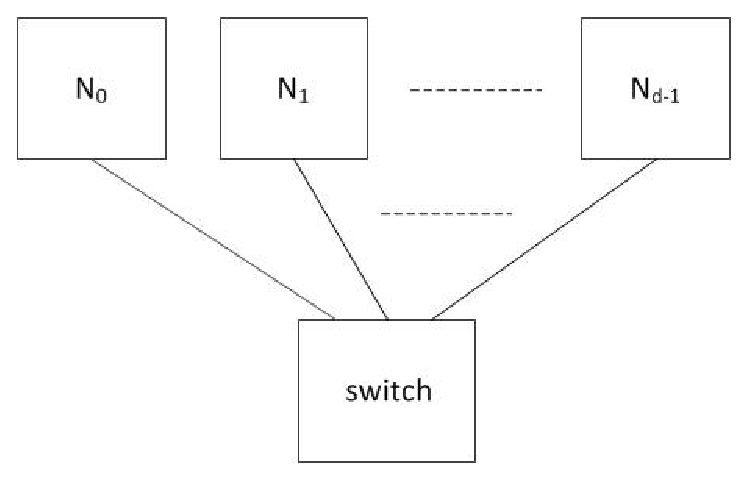
\includegraphics[width=0.4\textwidth]{distributed_system.eps}
  \caption{The distributed system. }
  \label{fig:distributed_system}
\end{figure}


\subsection{Details}

Remember that the algorithms lcpa-disk and lcpa-disk-m compute $ECP_{\log K}$ and $EPP_{\log K}$ via two runs of radix-sort in external memory. To emulate the procedure in the distributed system illustrated in Fig.\ref{fig:distributed_system}, we set up a group of sending/receiding buffers in each computing nodes for data transmission during the sorts.

{\color{red} Notice: refer to a line by a label, don't use a fixed number.}

Fig.~\ref{fig:alg:ds} shows that, in each round of the while-loop, lcpa-ds  performs two runs of radix-sorts to compute the $fp$ field of each entry in $ECP_k$ and $EPP_k$ by using the sending and receiving buffers in lines 7-15. Specifically, for each entry $x$ in $ECP_{i,k}$ ,$N_i$ dispatches $x$ to the sending buffer $SB1_{i,j}$ if $j = x.pos / e$ and delivers it to $RB1_{j,i}$ on $N_j$ in lines 7-8. Upon the arrival of each entry from the other nodes, $N_j$ caches the entry in its corresponding buffer in $\{RB1_{j,0},RB1_{j,1},...,RB1_{j,d-1}\}$ and then radix-sorts the received entries by $pos$ to form $IECP_{j,k}$ in lines 9-10. Then it scans $T_j$ from left to right for iteratively computing the fingerprints of the involved prefix substrings and record them in the $fp$ fields of the corresponding entries in $IECP_{j,k}$. Thereafter, in lines 12-13, each entry $y$ satisfying $i = y.pos /e$ is moved from $IECP_{j,k}$ to the sending buffer $SB1_{j,i}$ and then delivered to $RB1_{i,j}$ on $N_i$. Finally, $N_i$ radix-sorts the received entries in $\{RB1_{i,0},RB1_{i,1},...,RB1_{i,d-1}\}$ by their $idx$ to regenerate $ECP_{i,k}$ in lines 14-15. Note that the entries in $EPP_{i,k}$ can be processed using $\{SB2_{i,0}, SB2_{i,1},...,SB2_{i,d-1}\}$ and $\{RB2_{i,0}, RB2_{i,1}, ...,RB2_{i,d-1}\}$ in the same way as described above. Then, the algorithm generates $ECP_{i,k+1}$ and $EPP_{i,k+1}$ by scanning $ECP_{i,k}$ and $EPP_{i,k}$ once in line 16.

After the while-loop, the steps in lines 19-20 figure out the LCP-array of $T[ie,ie+e)$ in linear time from $ECP_{i,{\log K}}$, $EPP_{i,{\log K}}$ and $SA_{T_i}$ residing on $N_i$. Finally, we can simply collect and concatenate the LCP-array on each node to form $LCPA_T$.

\begin{algorithm}[t!]
\caption{Compute $K$-Order $LCPA_T[ie,ie+e)$ on $N_i$}
\label{fig:alg:ds}
lcpa-ds($T_i$, $SA_{T_i}$, $e$, $K$){\\
\SetAlgoNoLine
Scan $T_i$ rightward to compute $ECP_{i,0}$ and $EPP_{i,0}$. \\
Let $k=0$. \\
For $j\in[0,d)$, create sending buffers $SB1_{i,j}$ and $SB2_{i,j}$. \\
Create receiving buffers $RB1_i$ and $RB2_i$. \\
\While{$k < \log K$}{
\Indentp{-1em}
For $j\in[0,d)$ and $p\in[0,2e)$, scan $ECP_{i,k}$ and $EPP_{i,k}$ rightward to cache $ECP_{i,k}[p]$ in $SB1_{i,j}$ or $EPP_{i,k}[p]$ in $SB2_{i,j}$ if $ECP_{i,k}[p].pos$ or $EPP_{i,k}[p].pos$ belongs to $[je,je+e)$. \\
For $j\in[0,d)$, send entries in $SB1_{i,j}$ and $SB2_{i,j}$ to $N_j$. \\
For $j\in[0,d)$, cache entries from $SB1_{i,j}$ and $SB2_{i,j}$ in $RB1_i$ and $RB2_i$. \\
Radix-sort entries in $RB1_i$ and $RB2_i$ by $pos$ to produce $IECP_{i,k}$ and $IEPP_{i,k}$. \\
For $p\in[0,e)$ and $q\in [0,2e)$, scan $T_i$ rightward to iteratively compute the fingerprint of ${\sf pre}(T,ie+p)$ and assign $FP[0,ie+p]$ to $IECP_{i,k}[q].fp$ or $IEPP_{i,k}[q].fp$ if $IECP_{i,k}[q].pos = ie+p$ or $IEPP_{i,k}[q].pos = ie+p$. \\
For $j\in[0,d)$ and $p\in[0,2e)$, scan $IECP_i$ and $IEPP_i$ rightward to cache $IECP_{i,k}[p]$ in $SB1_{i,j}$ or $IEPP_{i,k}[p]$ in $SB2_{i,j}$ if $IECP_{i,k}[p].pos$ or $IEPP_{i,k}[p].pos$ belongs to $[je,je+e)$. \\
For $j\in[0,d)$, send entries in $SB1_{i,j}$ and $SB2_{i,j}$ to $N_j$. \\
For $j\in[0,d)$, cache entries from $SB1_{i,j}$ and $SB2_{i,j}$ in $RB1_i$ and $RB2_i$. \\
Radix-sort entries in $RB1_i$ and $RB2_i$ by $idx$ to reproduce $ECP_{i,k}$ and $EPP_{i,k}$. \\
For $p\in [0,e)$, scan $ECP_{i,k}$ and $EPP_{i,k}$ rightward to compute and compare the fingerprints of $T[ECP_{i,k}[2p].pos+1, ECP_{i,k}[2p+1].pos]$ and $T[EPP_{i,k}[2p].pos+1, EPP_{i,k}[2p+1].pos]$ for generating $ECP_{i,k+1}$ and $EPP_{i,k+1}$. \\
Let $k=k+1$. \\
}
For $p\in [0,e)$, scan $T_i$, $ECP_{i,\log K}$ and $EPP_{i,\log K}$ rightward to literally compute $\Upsilon_{i,p}={\sf lcp}(ECP_{i,\log K}[2p].pos,EPP_{i,\log K}[2p].pos)$. \\
For $p\in [0,e)$, let ${\sf lcp}(SA_{T_i}[p],SA_{T,i}[p-1])=ECP_{i,\log K}[2p].pos + \Upsilon_{i,p} - SA_{T_i}[p]$. \\
}
\end{algorithm}

The internal memory on each computing node is partitioned into two parts, where the first part is used to maintain the sending/receiving buffers and the other part is used to establish the I/O buffers for reading/writing and sorting the entries of $ECP_{i,k}$ and $EPP_{i,k}$. High performance can be achieved if these buffers are large enough to compensate the delay of data transmission and amortize the overhead of each I/O operation. It is noteworthy that the trick adopted in lcpa-disk-m can also be used herein to accelerate the running time with a growth in storage need {\color{red} (what do you mean? tell the trick clearly).}

{\color{red} ͻȻð������������û���νӡ�}

\begin{Lemma}
\label{thm:lcp:pdm}
Given $T$ and $SA_T$, the $K$-order $LCPA_T$ can be correctly computed in $\mathcal{O}(\frac{n}{d}\log K)$ time using $\mathcal{O}(\frac{n}{d})$ disk space on each computing node with a high probability.
\end{Lemma}
Proof. Algorithm~\ref{fig:alg:ds} performs radix-sorts {\color{red} (what?)} among the computing nodes, where the overhead of time and space for data transmission sums up to $\mathcal{O}(e\log K)$ during the whole loop, for each node sends and receives $\mathcal{O}(e)$ entries per round.



\section{Experimental Results}\label{sec:experimental_results}

A series of simulation experiments are conducted on a real data set collected from the web site \url{http://download.wikimedia.org/enwiki/} to evaluate our {C++} programs for the external and distributed algorithms presented in Section~\ref{sec:construction_in_em} and~\ref{sec:construction_in_distributed}, in terms of I/O volume, time consumption and peak disk use. Of our particular interest, we employ lcpa-disk-m as a baseline for performance assessment of lcpa-disk and investigate its scalability for a further study. The experimental platform for lcpa-disk and lcpa-disk-m is deployed on a computer equipped with 2 Intel Xeron E3-1220 CPUs, 4GB DDR3 main memory and a {(\color{red} 7200 or 5400rpm?)} 2TB disk, while the one for lcpa-ds is set up in a distributed system consisting of four identical computers interconnected with a gigabit switch. All the programs are compiled by gcc 4.8.4, and the operating system is Ubuntu 14.04.

STXXL is a {C++} STL library designed for efficient computations in external memory, freely available at \url{http://stxxl.sourceforge.net/}. Instead of to develop a radix sorter specific for our purpose, we use STXXL~\cite{Dementiev2007} to perform the external memory sorts in our programs. Specifically, a priority queue  provided by STXXL is employed for sorting the entries in $ECP_k/EPP_k$ by $pos$ to form $IECP_k/IEPP_k$ and another for sorting them back by $idx$. Benefit from the powerful priority queues, the codes for lcpa-disk, lcpa-disk-m and lcpa-ds are less than 400, 600 and 700 lines, respectively.

Each result in the following tables and figures is a mean of two runs of the programs, where the running time and peak disk use are monitored by the shell command ``time" and ``stxxl::block\_manager" provided by STXXL, respectively.

\subsection{Performance Analysis for External Algorithms}

The following parameters and metrics are used for the performance evaluation of our programs:
\begin{itemize}
\item $S$: corpora size.
\item $ST$: total running time.
\item $MT$: average running time spent in processing a character per loop round.
\item $PD$: peak disk use.
\item $LR$: number of loop rounds.
\item $W$: every $W$ successive loop rounds in lcpa-disk are merged into one in lcpa-disk-m.
\item $H$: internal memory allocated to each priority queue when sorting entries in external memory.
\end{itemize}

To show the effect of $W$, we demonstrate in Table.~\ref{tbl:disk_vs_diskm} the experimental results of lcpa-disk and lcpa-disk-m. As can be seen, lcpa-disk-m has a smaller $ST$ than lcpa-disk when $W=2$, while the latter outperforms the former in terms of $MT$ and $PD$ under the same circumstances. Specifically, given $K=8192$, the speed of lcpa-disk-m for $W=2$ is nearly one-third faster than that of lcpa-disk when $S$ varies from 200 MB to 2 GB. However, the total running time of lcpa-disk-m for $W=3$ grows rapidly as $S$ increases and exceeds the counterpart of lcpa-disk when $S$ ascends to 2 GB. This behavior can be explained as following. As described in Section~\ref{sec:construction_in_em}, lcpa-disk-m can merge every $W$ successive loop rounds for decreasing $LR$ by computing all the fingerprints possibly involved in $W$ successive loop rounds. For example, given $W=2$ and $W=3$, lcpa-disk-m maintains 3 and 7 fingerprints in each entry of $ECP_k$ and $EPP_k$, respectively, and updates them during each loop round. This leads to a sharp growth in the computation and I/O overhead per round against lcpa-disk and becomes a performance bottleneck.

Fig.~\ref{fig:disk_vs_diskm} illustrates the variation trend of $MT$ with increasing $S$. The non-linear relationship between the two parameters violates the assumption that $MT$ is linear proportional to $S$. This behavior is partly due to the use of STXXL, where the priority queue provided by the library takes logarithmic time to sort elements in external memory.

\begin{table*}[htbp!]
\caption{$LR$, $MT$ in microseconds per (character $\cdot$ round), $ST$ in seconds and $PD$ in bytes per character, where $K=8192$, $W$ ranges in $\{2,3\}$ and $S$ varies from 200 MB to 2 GB.}
\label{tbl:disk_vs_diskm}
\centering
\begin{tabular}{|c|c|c|c|c|c|c|c|c|c|c|c|c|}
\hline
$S$ & \multicolumn{4}{c|}{lcpa-disk} & \multicolumn{4}{c|}{lcpa-disk-m ($W = 2$)} & \multicolumn{4}{c|}{lcpa-disk-m ($W = 3$)}\\
\cline{2-13}
(MB) & $LR$ & $MT$ & $ST$ & $PD$ & $LR$ & $MT$ & $ST$ & $PD$ & $LR$ & $MT$ & $ST$ & $PD$\\
\hline
200 & 13 & 1.03 & 2803 & 30.94 & 7 & 1.33 & 1950 & 47.36 & 5 & 2.43 & 2541 & 77.52\\
\hline
400 & 13 & 1.11 & 6034 & 31.50 & 7 & 1.40 & 4108 & 47.36 & 5 & 2.20 & 4605 & 78.58\\
\hline
600 & 13 & 1.18 & 9650 & 31.58 & 7 & 1.48 & 6928 & 47.36 & 5 & 3.14 & 9860 & 130.86\\
\hline
800 & 13 & 1.34 & 14557 & 31.52 & 7 & 1.80 & 10547 & 47.38 & 5 & 3.06 & 12827 & 103.50\\
\hline
2048 & 13 & 1.72 & 48021 & 46.04 & 7 & 2.47 & 37029 & 60.48 & 5 & 4.59 & 49280 & 94.40\\
\hline
\end{tabular}
\centering
\end{table*}

\begin{table*}[htbp!]
\caption{$LR$, $MT$ in microseconds per (character $\cdot$ round), $ST$ in seconds and $PD$ in bytes per character, where $K=8192$, $N=4$, $W=2$ and $S$ varies from 200 MB to 2 GB.}
\label{tbl:diskm_vs_ds}
\centering
\begin{tabular}{|c|c|c|c|c|c|c|c|c|}
\hline
$S$ & $LR$ & \multicolumn{3}{c|}{lcpa-ds~($N=4$)} & \multicolumn{3}{c|}{lcpa-disk-m} & Speedup\\
\cline{3-8}
(MB) & & $MT$ & $ST$ & $PD$ & $MT$ & $ST$ & $PD$ & (\%)\\
\hline
200 & 7 & 0.71 & 1038 & 13.50 & 1.33 & 1950 & 47.36 & 0.54 \\
\hline
400 & 7 & 0.72 & 2113 & 13.50 & 1.40 & 4108 & 47.36 & 0.52 \\
\hline
600 & 7 & 0.74 & 3235 & 13.75 & 1.48 & 6928 & 47.36 & 0.50 \\
\hline
800 & 7 & 0.78 & 4547 & 13.82 & 1.80 & 10547 & 47.38 & 0.43 \\
\hline
2048 & 7 & 1.24 & 18617 & 16.21 & 2.47 & 37029 & 60.48 & 0.50 \\
\hline
\end{tabular}
\centering
\end{table*}

\begin{figure}[hbtp!]
  \centering
  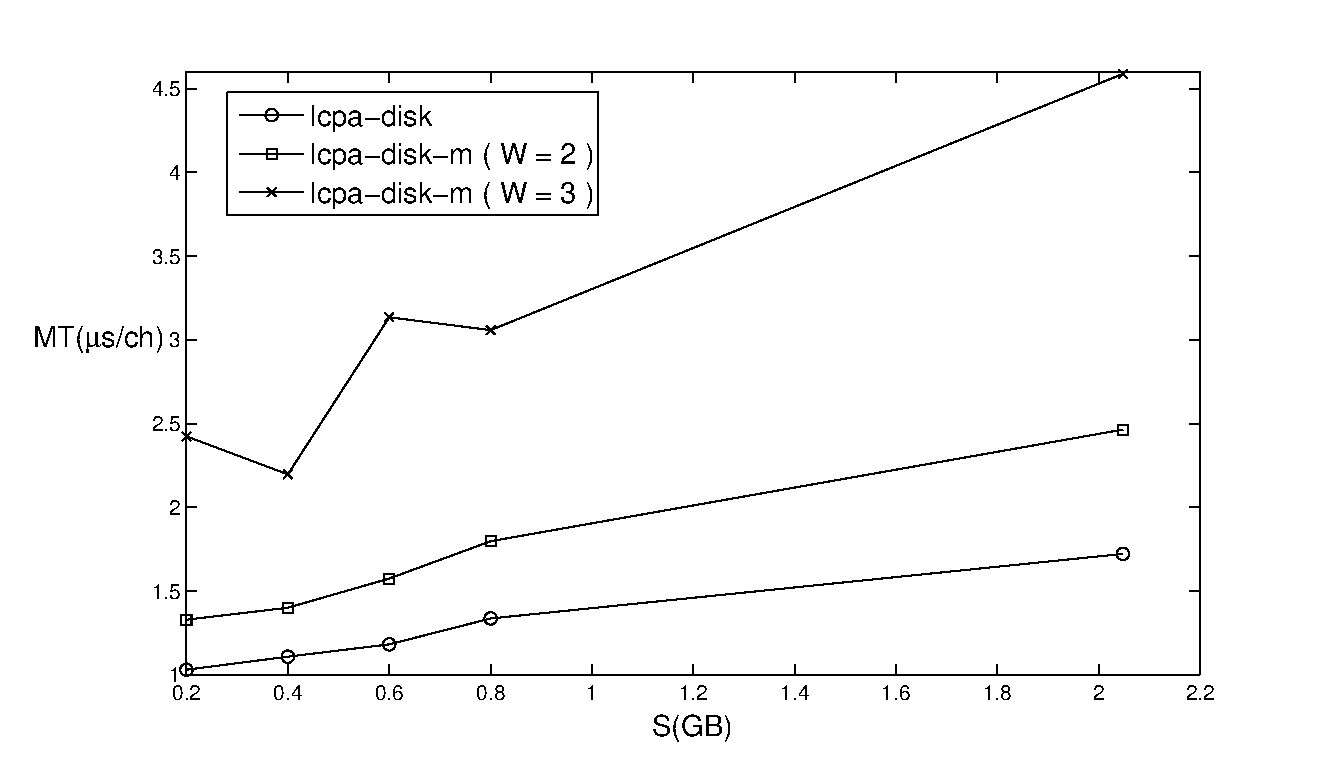
\includegraphics[width=0.5\textwidth]{disk_vs_diskm.eps}
  \caption{Performance comparison for lcpa-disk and lcpa-disk-m with $S$ varying from 0.2 to 2 GB, where $K=8192$ and $W=2$.}
  \label{fig:disk_vs_diskm}
\end{figure}

{\color{red} The figures are too short, the fonts are two small.}

As reported in~\cite{Juha2014}, the disk space requirements for eSAIS and LCPscan are $65n$ and $21n$, respectively, while the peak disk use of our implementation for lcpa-disk-m~($W=2$) rises up to $61n$ for processing a 2 GB corpora. This indicates that {lcpa-disk-m} is more space demanding compared with the current best methods. However, we will show in the following that our method is easy to be implemented and strongly scalable for parallel and distributed models where the communication overhead on each node is balanced as $\mathcal{O}(\frac{n}{d})$.


\subsection{Performance Analysis for Distributed Algorithms}

The algorithm lcpa-ds can be naturally executed in parallel except for the external memory sorts, showing a feature of strong scalability. We have described in Section~\ref{sec:construction_in_distributed} how to emulate the sorter by using a group of sending/receiving buffers. The communication overhead of each computing node in~Fig.~\ref{fig:distributed_system} is upper-bounded by $\mathcal{O}(e)$. According to Amdahl's Law, the theoretical speed of lcpa-ds is $N-1$ times faster than that of lcpa-disk, where $N$ is the number of computing nodes in the distributed system. To validate the point, we provide lcpa-disk-m as a baseline to evaluate the performance of lcpa-ds.

As described in Table.~\ref{tbl:diskm_vs_ds}, lcpa-ds outperforms lcpa-disk-m in terms of $MT$ and $ST$ by a factor of 2, where $K=8192$, $W=2$ and $N=4$. Particularly, $MT$ for lcpa-ds increases from 0.71 to 1.24 when $S$ increases from 200 MB to 2 GB. However, the performance gain does not meet our expectation. One factor to {\color{red} ???} the problem lies in the parallel overhead for data transmission among the computing nodes, but the major reason is due to the insufficient internal memory. In details, each computing node takes half the internal memory for maintaining the sending/receiving buffers and uses the remaining part for establishing the I/O buffers. Particularly, it is memory-intensive when sorting the entries in external memory, as each priority queue creates a heap to amortize the overhead of disk accesses. Fig.~\ref{fig:stxxl_pq_impact} shows the negative impact to $MT$ where $H$ decreases from 1.35 to 0.5 GB, given $S$ in $\{400, 800, 2048\}$ MB.

\begin{figure}[hbtp!]
  \centering
  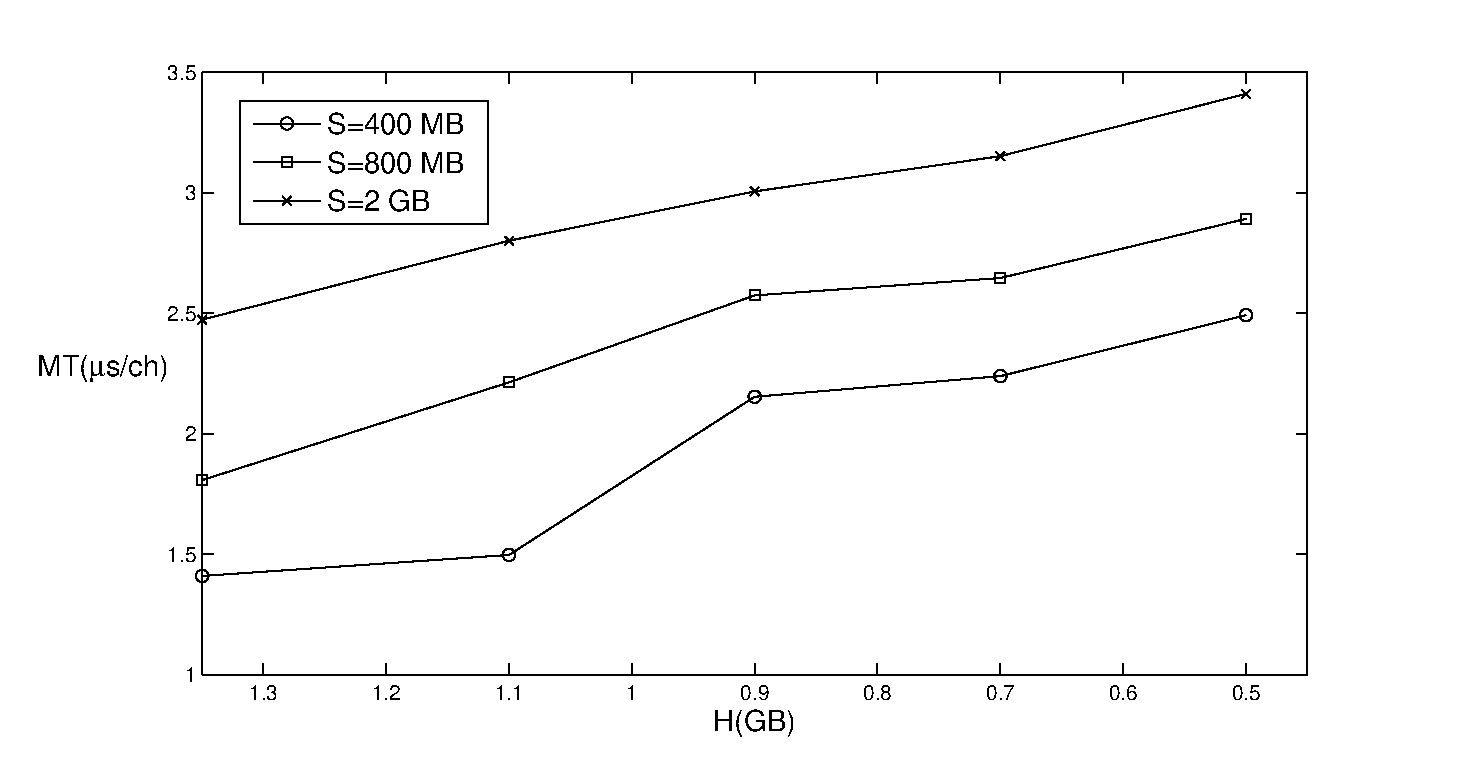
\includegraphics[width=0.5\textwidth]{stxxl_pq_impact.eps}\\
  \caption{Performance analysis for lcpa-disk-m with $H$ varying from 1.35 to 0.5 GB, where $K=8192$, $W=2$, $N=4$ and $S$ in $\{400, 800, 2048\}$ MB.}
  \label{fig:stxxl_pq_impact}
\end{figure}

To further evaluate the scalability of lcpa-ds, we show in Fig.~\ref{fig:ds_varying_n} the variation trend of $MT$ against $N$. It can be observed that $MT$ becomes smaller and grows more smoothly with larger $N$.

\begin{figure}[hbtp!]
  \centering
  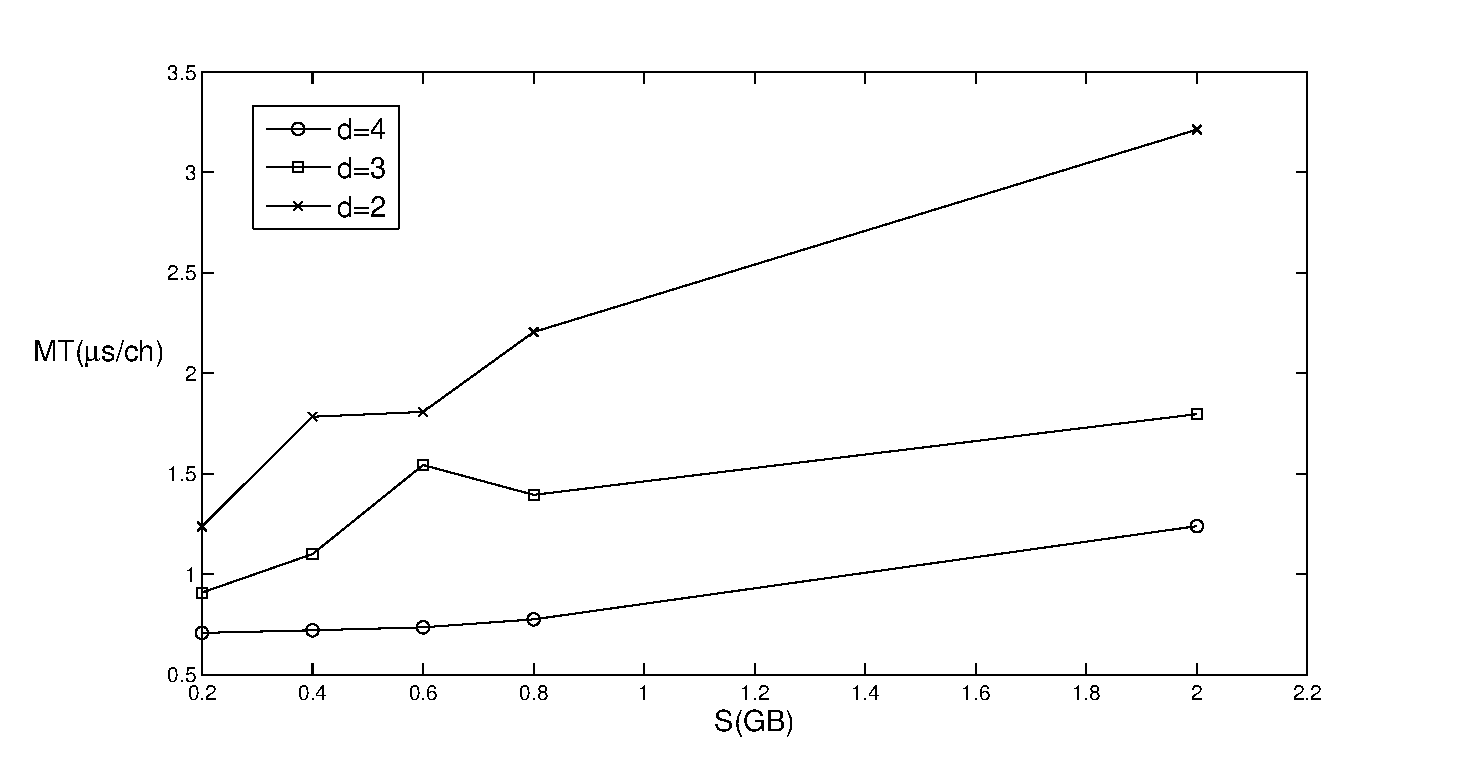
\includegraphics[width=0.5\textwidth]{ds_varying_n.eps}\\
  \caption{Performance analysis for lcpa-ds with $S$ varying from 0.2 to 2 GB, where $K=8192$, $W=2$ and $N$ in $\{2,3,4\}$.}
  \label{fig:ds_varying_n}
\end{figure}


\section{Conclusion}\label{sec:conclusion}

We present in this paper a practical $K$-order LCP-array construction method that can be easily applied on both the internal memory and the external memory models. The program for lcpa-disk-m is less than 600 lines when using STXXL to implement the external sorts. We also show that the proposed method is straightforward to be extended for running on a typical distributed system of a cluster of $d$ computing nodes, where the time and space complexities are evenly divided onto each node as $\mathcal{O}(\frac{n}{d}\log K)$ and $\mathcal{O}(\frac{n}{d})$, respectively. The proposed algorithms are simple in design and universal for the RAM, disk and distributed models. Its implementations on all these models are not difficult and easily to be deployed.
A cluster of computers in a local area network are commonly available in practice, but there are currently lack of scalable LCP-array construction algorithms for such a distributed model. In this sense, our algorithms provide a candidate solution to meet the demand. For further work, we now attempt to speed up the computation of fingerprints by GPU.

\section*{Acknowledgment}
The work of Ge Nong is partially supported by The DEGP of China (grant no. 2012KJCX0001). The work of Wai Hong Chan is supported by The Research Grant Council of Hong Kong SAR (grant no. GRF 810012).

\bibliographystyle{unsrt}
\bibliography{bibfile}

\end{CJK*}
\end{document}


